\documentclass{article}
\usepackage{hyperref}
\usepackage{graphicx}
\usepackage{subfigure}
\usepackage[a4paper, total={6in, 8in}]{geometry}
\title{Khidmat Bird Recogntion Project\\ \textit{Intemediate Progress Report}}
\author{Ali Hamza}
\date{\today}

\begin{document}

    \maketitle
    \section*{Introduction}
    \subsection*{Objective}
    The objective of this Khidmat as dicussed initially with WWF representaties is create a machine learning algorithm that distinguishes between 3 birds that will act as the first stage indeveloping a larger ML model for the WWF app for recognizing birds. The 3 birds chosen for the scope of this project are the Common Myna, Housesparrow, and Housecrow - this project ultimately serves as a proof of concept and a test of the ability to build a model that can distinguish between birds.

    \section*{Methodology}
    The following steps were initially established in order to achieve this objective:
    
    \begin{enumerate}
        \item Image collection
        \item Image preprocessing
        \item Feature extraction
        \item Training
        \item Testing
        \item Results
        \item Conclusion
    \end{enumerate}

    \subsection*{Image Collection}
    The images were collected from the following websites:
    \begin{enumerate}
        \item \url{https://search.macaulaylibrary.org/catalog?taxonCode=myna&mediaType=p&q=Common%20Myna}
        \item \url{https://ebird.org/media/catalog?taxonCode=commyn&mediaType=p&sort=rating_rank_desc&q=Common%20Myna%20-%20Acridotheres%20tristis}
        \item \url{https://ebird.org/media/catalog?taxonCode=houcro1&sort=rating_rank_desc&mediaType=p&regionCode=}
        \item \url{https://search.macaulaylibrary.org/catalog?taxonCode=houcro1&mediaType=p&region=Pakistan%20(PK)&regionCode=PK&q=House%20Crow%20-%20Corvus%20splendens}
        \item \url{https://www.kaggle.com/gpiosenka/100-bird-species}
        \item \url{https://search.macaulaylibrary.org/catalog?taxonCode=houspa&mediaType=p&q=House%20Sparrow}
        \item \url{https://ebird.org/media/catalog?taxonCode=houspa&mediaType=p&sort=rating_rank_desc&q=House%20Sparrow%20-%20Passer%20domesticus}
    \end{enumerate}     
    % All the images that were collected have been stored on \hyperref[]https://drive.google.com/drive/folders/18k-roE_VJSB1dcrhvN1y_EosVF7Kb0dY?usp=sharing]{Google Drive}
    All images collected: \url{https://drive.google.com/drive/folders/18k-roE_VJSB1dcrhvN1y_EosVF7Kb0dY?usp=sharing}
    \subsection*{Image Preprocessing}
    The images were preprocessed using the following steps:
    \begin{enumerate}
        \item \texttt{Find Box} Function \newline 
        Each image was taken an a Computer Vision tool was used to find a box that contains a bird-like object within it. This function would then detect all edges of the bounding-box the bird-like object has been detected to be inside. This ensure the final image only contains the bird itself.
        \item \texttt{Crop Image} Function  \newline
        Each image was then taken and cropped into a square as this would standardize each image that will be fed into the neural net. We cropped images to sizes: $50\times 50$, $100\times 100$, and $200\times 200$ as seen in \ref{Birds}
    \end{enumerate}


    \subsection*{Feature Extraction}
    The following features were extracted from the images:
    % \begin{enumerate}
        % \item Color Histogram
        % \item Color Layout
        % \item Color Layout Variance
        % \item Color Layout Entropy
        % \item Color Layout Difference
    % \end{enumerate}

    \subsection*{Training}
    The following algorithm was used to train the model:
    

    \subsection*{Testing}
    The following algorithm was used to test the model:
    
    \subsection*{Results}
    The following algorithm was used to test the model:
    
    \subsection*{Conclusion}
    
    This pipeline with certain configuration yielded a detection accuracy of 87$\%$


    \section*{Remaining Work}
    
    Based on our recent interactiong with Dr. Sarah Husnain, we've decided to that the model can be made to be slightly more accurate and reach at least $\%$ accuracy. This can be done by taking the following steps:
    \begin{enumerate}
        \item Collecting at least 50-60 more images of each bird
        \item Augmentation of the data
        \item Further fine-tuning of Parameters
    \end{enumerate}
    The final model will be trained on the entire dataset and tested again. We further plan to createt a detailed report at the end of this project for WWF, Pakistan detailing each component of the machine learning pipe line. The report will serve as a record of the work done, and a manual for the future developers to follow.
    
    \section*{Addendum}
    \subsection*{Code}
    \subsection*{Results}
    \subsection*{Figures and Images}
        \begin{figure}[h!]
        \centering
        \subfigure[$50\times 50$]{
        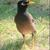
\includegraphics[]{pictures/CM1.jpg}
        }
        \subfigure[$100\times 100$]{
        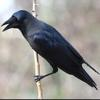
\includegraphics[]{pictures/HC4.jpg}
        }
        \subfigure[$200\times 200$ ]{
        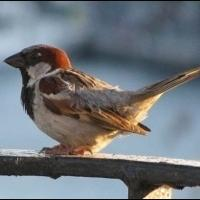
\includegraphics[]{pictures/HS2.jpg}
        }
        \caption{Preprocessed Bird Images}
        \label{Birds}
    \end{figure}
   
        
        
\end{document}

